Xu grep is an extension of the usual grep to permit it to pass from text processing to context free. A use case for this to get a function name as function without getting all mentions of the function the comments. So just grepping more precisely.
Command example:
\begin{lstlisting}[language=bash]
   xugrep.py [xupath] [input file]
\end{lstlisting}

xupath: is a gseneralisation of xpath. It is needed as xugrep works with hierarchichal object models.
Example usage can be seen in this figure \ref{fig:example1xugrep}.

\begin{figure}
\label{fig:example1xugrep}
\caption{Function name in a file. Used a C file.}
\includegraphics[width=\textwidth]{images/example1xugrep.jpg}
\end{figure}

In figure \ref{fig:example2xugrep} you can see a second example. This is for searching within a IOS interface config file.

\begin{figure}
\label{fig:example2xugrep}
\caption{Extracting IOS Interfaces}
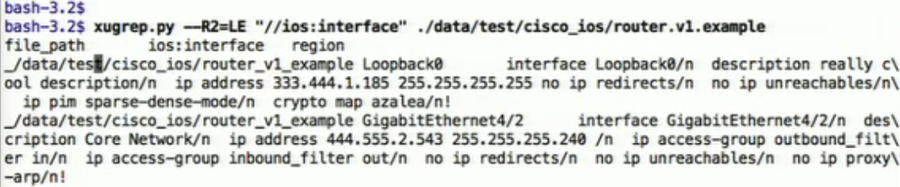
\includegraphics[width=\textwidth]{images/example2xugrep.png}
\end{figure}

In the last figure you can how the xu grep searches for all the Interfaces in a Cisco IOS config file. In figure \ref{fig:example3xugrep} you can see the illustration.
\begin{enumerate}
\item Look through all the given input files.
\item Look for all the interfaces within these files
\item Output all that you have found. 
\end{enumerate}

\begin{figure}
\label{fig:example3xugrep}
\caption{Search tree for interface Cisco IOS}
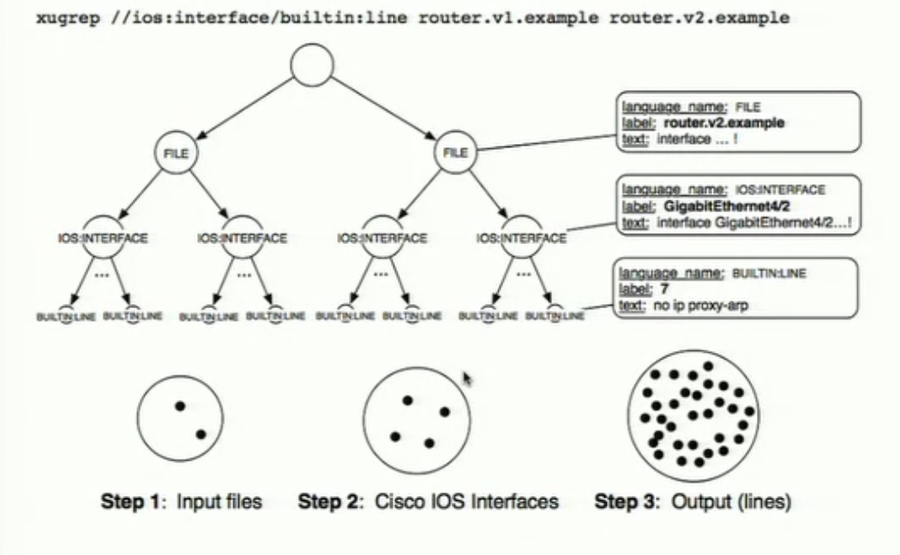
\includegraphics[width=\textwidth]{images/example3xugrep.png}
\end{figure}